\vspace*{-4cm}
\chapter{Análisis}
\label{ch:analisis}

En este capítulo se presenta el desglose formal de las necesidades del sistema AUTECH mediante la especificación de sus requerimientos funcionales y no funcionales, el establecimiento de sus reglas de negocio, y el modelado detallado de sus casos de uso bajo el estándar UML.

\section{Requerimientos Globales del Sistema (IEEE 830)}
\label{sec:ieee830}

La especificación de requisitos se fundamenta en la norma IEEE Std 830-1998, asegurando una trazabilidad bidireccional y una comunicación sin ambigüedades entre la arquitectura de software y las necesidades didácticas institucionales \cite{ieee1998}.

\subsection{Requerimientos Funcionales}
\label{subsec:req_funcionales}

Los requerimientos funcionales (RF) definen el comportamiento interno del sistema, las transformaciones de datos y los servicios directos que se proveen a los distintos perfiles de usuario. Para garantizar la cohesión del diseño, se han classified en cuatro módulos arquitectónicos, como se definen en la Tabla~\ref{tab:rf_sistema} y la Tabla~\ref{tab:rf_sistema_p2}.

\begin{table}[htbp]
    \centering
    \small
    \caption{Requerimientos Funcionales del Sistema AUTECH, organizados en cuatro módulos: Gestión y Seguridad (RF-01 a RF-03), Simulación y Motor Algorítmico (RF-04 a RF-08), Didáctico y de Ludificación (RF-09 a RF-12) e Interoperabilidad y UX (RF-13 a RF-15).}
    \label{tab:rf_sistema}
    \begin{tabular}{l l p{9.5cm}}
        \toprule
        \textbf{ID} & \textbf{Nombre del Requerimiento} & \textbf{Especificación Técnica} \\
        \midrule
        \multicolumn{3}{l}{\textbf{MÓDULO DE GESTIÓN Y SEGURIDAD}} \\
        \midrule
        RF-01 & Gestión Multi-Rol & Administrar el control de acceso de manera multiplataforma y concurrente para tres perfiles jerárquicos: Administrador (gestión global), Docente (gestión académica) y Alumno (simulación) \cite{pressman2020}. \\
        \addlinespace
        RF-02 & Aprovisionamiento Docente & Permitir el envío de solicitudes de registro docente. Tras la validación del Administrador (vía entorno desktop o móvil), el sistema deberá aprovisionar la cuenta automatizando el envío de credenciales temporales vía correo electrónico. \\
        \addlinespace
        RF-03 & Gestión de Grupos Académicos & Proveer al perfil Docente de un panel de control disponible en plataformas desktop y móvil para crear, modificar o eliminar grupos, así como generar identificadores alfanuméricos (códigos de invitación) para el enrolamiento de alumnos \cite{escom2016}. \\
        \midrule
        \multicolumn{3}{l}{\textbf{MÓDULO DE SIMULACIÓN Y MOTOR ALGORÍTMICO}} \\
        \midrule
        RF-04 & Editor de Autómatas Finitos & Desplegar un canvas interactivo en la aplicación móvil que permita la construcción y edición topológica de Autómatas Finitos Deterministas (AFD) y No Deterministas (AFND) \cite{ipn2020}. \\
        \addlinespace
        RF-05 & Editor de Autómatas de Pila & Proveer herramientas de diseño para Autómatas de Pila (AP) en la interfaz móvil, integrando la declaración del alfabeto de la pila ($\Gamma$) y la gestión de transiciones no deterministas \cite{hopcroft2007}. \\
        \addlinespace
        RF-06 & Editor de Máquinas de Turing & Desplegar en la aplicación móvil un simulador de Máquina de Turing (MT) orientado a la función de reconocimiento de lenguajes, incorporando una cinta infinita visual y control de cabezal bidireccional \cite{sipser2012}. \\
        \addlinespace
        RF-07 & Validador Lógico Multinivel & Ejecutar la validación algorítmica de cadenas de entrada en tres modalidades asíncronas: 1) Ejecución paso a paso, 2) Resolución de clausuras épsilon ($\epsilon$), y 3) Evaluación masiva de baterías de prueba (\textit{Bulk Test}) \cite{sinchi2018}. \\
        \addlinespace
        RF-08 & Transformación Algorítmica & Ejecutar conversiones matemáticas automatizadas, incluyendo: transformación de AFND a AFD, minimización de estados equivalentes y conversión bidireccional entre Expresiones Regulares y grafos \cite{kelley2001}. \\
        \bottomrule
    \end{tabular}
\end{table}

\begin{table}[htbp]
    \centering
    \small
    \caption{Requerimientos Funcionales del Sistema AUTECH (Continuación).}
    \label{tab:rf_sistema_p2}
    \begin{tabular}{l l p{9.5cm}}
        \toprule
        \textbf{ID} & \textbf{Nombre del Requerimiento} & \textbf{Especificación Técnica} \\
        \midrule
        \multicolumn{3}{l}{\textbf{MÓDULO DIDÁCTICO Y DE LUDIFICACIÓN}} \\
        \midrule
        RF-09 & Evaluaciones Teóricas (Quizzes) & Permitir la creación y asignación multiplataforma de reactivos de opción múltiple orientados exclusivamente a la validación de fundamentos teóricos de la asignatura \cite{felder2016}. \\
        \addlinespace
        RF-10 & Analítica de Desempeño Docente & Procesar las métricas de uso y generar visualizaciones estadísticas (indicadores semaforizados) del avance grupal e individual (aciertos, errores frecuentes y completitud temporal) accesibles para el profesor \cite{munoz2012}. \\
        \addlinespace
        RF-11 & Ecosistema de Ludificación & Orquestar el progreso del usuario mediante el bloqueo/desbloqueo de ``mundos'' basados en la Jerarquía de Chomsky, calculando puntos de experiencia (XP) y gestionando contadores de racha de estudio en la app móvil del Alumno \cite{deterding2011}. \\
        \addlinespace
        RF-12 & Integración Multimedia & Integrar y reproducir material audiovisual de refuerzo desde fuentes externas de manera adaptativa en la interfaz móvil \cite{crompton2018}. \\
        \midrule
        \multicolumn{3}{l}{\textbf{MÓDULO DE INTEROPERABILIDAD Y UX}} \\
        \midrule
        RF-13 & Interoperabilidad de Estructuras & Soportar la importación y exportación bidireccional del mapeo de grafos utilizando los esquemas XML estándar de la industria académica: \texttt{.jff} (JFLAP) y \texttt{.fsam} a través del gestor de archivos nativo de cada entorno \cite{rodger2006}. \\
        \addlinespace
        RF-14 & Asistente de Inducción (Onboarding) & Desplegar una secuencia de instrucciones superpuestas e interactivas al detectar el primer inicio de sesión en la aplicación móvil del Alumno, con capacidad de ser omitida por el usuario \cite{materialdesign2023}. \\
        \addlinespace
        RF-15 & Modo de Práctica Autónoma & Habilitar el acceso irrestricto en la app móvil a los módulos de simulación y lecciones teóricas para cuentas de Alumno que no estén vinculadas a un código de grupo docente \cite{nielsen1994}. \\
        \bottomrule
    \end{tabular}
\end{table}

\newpage
\subsection{Requerimientos No Funcionales (RNF)}
\label{subsec:req_no_funcionales}

Los requerimientos no funcionales (RNF) especifican las restricciones técnicas, criterios de calidad del sistema, directrices de seguridad y métricas de rendimiento indispensables para garantizar el correcto funcionamiento transversal de la arquitectura de AUTECH, detallados en la Tabla~\ref{tab:req_no_funcionales}.

\begin{table}[htbp]
    \centering
    \small
    \caption{Especificación de Requerimientos No Funcionales del Ecosistema AUTECH.}
    \label{tab:req_no_funcionales}
    \begin{tabular}{l l p{9.5cm}}
        \toprule
        \textbf{ID} & \textbf{Atributo de Calidad} & \textbf{Especificación y Restricción Técnica} \\
        \midrule
        RNF-01 & Rendimiento Gráfico & El renderizado y la animación matemática de los grafos sobre el canvas interactivo en Flutter debe mantener una tasa de refresco estable de 60 FPS tanto en dispositivos móviles como en entornos Desktop (Windows/macOS) \cite{flutter2024a}. \\
        \addlinespace
        RNF-02 & Persistencia Local Móvil & La lectura y escritura de estructuras de autómatas y progreso local en la aplicación móvil del Alumno debe realizarse mediante cajas no relacionales de Hive, garantizando tiempos de respuesta inferiores a los 15 ms. \\
        \addlinespace
        RNF-03 & Resiliencia Offline & El cliente móvil del Alumno debe procesar el cambio dinámico de red mediante un Service Layer reactivo, encolando localmente las peticiones de sincronización en background al perder de forma temporal la conectividad \cite{flutter2024c}. \\
        \addlinespace
        RNF-04 & Disponibilidad de API & La API de servicios web desplegada en la infraestructura en la nube de Render debe responder eficientemente a las peticiones concurrentes de las aplicaciones, garantizando un \textit{uptime} del 99.5\% anual. \\
        \addlinespace
        RNF-05 & Seguridad y Cifrado & Todo flujo de datos e intercambio de información entre los clientes de software (móviles o desktop) y la base de datos centralizada debe realizarse obligatoriamente mediante peticiones cifradas bajo el protocolo HTTPS (TLS 1.3). \\
        \addlinespace
        RNF-06 & Seguridad en Capa de Datos & El acceso a la persistencia en la nube debe controlarse estrictamente a través de políticas de seguridad a nivel de fila (RLS, \textit{Row Level Security}) vinculadas al ID único de usuario de la sesión activa en cualquier plataforma \cite{supabase2024}. \\
        \addlinespace
        RNF-07 & Escalabilidad Concurrente & El esquema de base de datos relacional y el pool de conexiones del backend deben estar dimensionados para soportar consultas simultáneas provenientes de múltiples peticiones concurrentes en periodos de evaluación masiva bajo estándares internacionales de calidad \cite{iso2011}. \\
        \bottomrule
    \end{tabular}
\end{table}

\clearpage
\section{Reglas de Negocio}
\label{sec:reglas_negocio}

Las reglas de negocio definen las políticas, restricciones lógicas y leyes matemáticas constantes, que el sistema debe respetar durante su ejecución. A diferencia de los requerimientos funcionales, estas reglas aseguran que la simulación gráfica sea matemáticamente exacta y que el avance del estudiante sea didácticamente coherente con el programa de estudios \cite{ipn2020, hopcroft2007}. La especificación detallada de estas directrices se presenta en la Tabla~\ref{tab:reglas_negocio}.

\begin{table}[htbp]
    \centering
    \small
    \caption{Reglas de Negocio del Sistema AUTECH.}
    \label{tab:reglas_negocio}
    \begin{tabular}{l l p{9.5cm}}
        \toprule
        \textbf{ID} & \textbf{Nombre de la Regla} & \textbf{Restricción Lógica y Matemática} \\
        \midrule
        RN-01 & Determinismo Estricto (AFD) & Durante la edición de un Autómata Finito Determinista, el sistema impedirá la ejecución de la simulación y desplegará una alerta de error si detecta que un estado posee múltiples transiciones de salida evaluadas con el mismo símbolo del alfabeto \cite{hopcroft2007}. \\
        \addlinespace
        RN-02 & Integridad de Memoria LIFO & En el simulador de Autómatas de Pila, el motor de validación prohibirá cualquier operation de extracción (POP) si el estado actual de la pila contiene únicamente el símbolo de fondo inicial ($Z_0$), evitando desbordamientos lógicos \cite{hopcroft2007}. \\
        \addlinespace
        RN-03 & Límite Físico de Cinta (MT) & Conforme al modelo estándar de Máquina de Turing de cinta semi-infinita, el sistema restringirá el desplazamiento del cabezal hacia la izquierda si su posición actual corresponde a la celda de inicio (índice cero) \cite{hopcroft2007}. \\
        \addlinespace
        RN-04 & Umbral de Competencia Didáctica & El sistema aplicará un candado lógico que impedirá el desbloqueo de un nivel superior (por ejemplo, la transición de Lenguajes Regulares a Libres de Contexto) a menos que el usuario acredite el módulo vigente con un puntaje mínimo aprobatorio de 80/100. La implementación de esta regla corresponde al Ciclo 1 del prototipado evolutivo, una vez que el sistema de progresión base quede consolidado en el Ciclo 0 \cite{ipn2020}. \\
        \addlinespace
        RN-05 & Límite de Complejidad Topológica & Para mantener el alineamiento con el RNF-01 de rendimiento, el lienzo de simulación emitirá una advertencia preventiva de optimización si la topología del grafo diseñado por el usuario alcanza los 15 estados activos. \\
        \addlinespace
        RN-06 & Iteración Formativa Ilimitada & El sistema garantizará que las cuentas con rol de Alumno posean intentos infinitos para la resolución de simulaciones y cuestionarios teóricos, priorizando la internalización del conocimiento por repetición sobre la penalización punitiva. \\
        \bottomrule
    \end{tabular}
\end{table}

\clearpage 

\section{Especificación de Requisitos y Modelado Funcional (UML)}
\label{sec:especificacion_uml}

La ingeniería de requisitos visual permite modelar las limitaciones operativas del sistema, facilitando la comprensión de los flujos de trabajo sin comprometerse con detalles de implementación a nivel de código. Para mantener el rigor técnico exigido en el IPN, se utiliza el estándar industrial UML 2.5 (Lenguaje de Modelado Unificado), el cual esquematiza cómo las entidades humanas interactúan con los procesos de la Jerarquía de Chomsky y el motor analítico del sistema \cite{pressman2020}.

\subsection{Actores del Sistema}
\label{subsec:actores_sistema}

De acuerdo con las especificaciones de UML 2.5, un ``Actor'' representa un rol que desempeña un usuario humano o un sistema externo al interactuar con el caso de uso \cite{pressman2020}. Para AUTECH, se han definido estrictamente tres perfiles jerárquicos basados en una arquitectura de control de acceso por roles (RBAC) \cite{supabase2024}.

\begin{quote}
    \small \textit{\textbf{Nota Técnica de Arquitectura:} Se omite deliberadamente la inclusión de componentes de infraestructura interna, como la base de datos local Hive o el proveedor de autenticación Supabase Auth, ya que no inician interacciones de forma autónoma, sino que responden a peticiones del cliente.}
\end{quote}

\begin{description}
    \item[\textbf{Alumno (Actor Primario - Móvil):}] Estudiante matriculado en la ESCOM. Su objetivo principal es interactuar exclusivamente con el cliente móvil (Android) para resolver simulaciones de autómatas, consultar teoría algorítmica y gestionar su progresión académica dentro del ecosistema ludificado \cite{ipn2020, materialdesign2023}.
    \item[\textbf{Docente (Actor Primario - Multiplataforma adaptativo Desktop/Móvil):}] Profesor titular de la asignatura de Teoría de la Computación. Su interacción se centraliza en el Dashboard Desktop y dispositivos móviles, donde ejerce funciones de evaluación formativa, gestión de grupos académicos (códigos de invitación) y análisis de métricas de desempeño \cite{felder2016}.
    \item[\textbf{Administrador (Actor Secundario - Multiplataforma adaptativo Desktop/Móvil):}] Perfil técnico y operativo con privilegios globales (\textit{Super User}). Su responsabilidad recae en el aprovisionamiento de cuentas institucionales (validación y aprobación de registros docentes) y el mantenimiento de los parámetros de configuración globales del sistema \cite{supabase2024}.
\end{description}
\subsection{Casos de Uso}
\label{subsec:casos_uso}

El catálogo de Casos de Uso (CU) define las interacciones entre los actores (Alumno, Docente, Administrador) y los servicios del sistema, clasificando cada función por su importancia para el proceso educativo (Prioridad) y su impacto en la estabilidad del software (Criticidad). Los casos de uso se derivan de las funcionalidades implementadas en Flutter/Dart utilizando Supabase como plataforma de servicios backend.

Para optimizar la trazabilidad y ofrecer una visión holística del sistema, el catálogo completo de AUTECH se ha unificado en la Tabla~\ref{tab:catalogo_cu_consolidado} y la Tabla~\ref{tab:catalogo_cu_consolidado_p2}, segmentado jerárquicamente por el ámbito de aplicación de cada módulo y ordenado en una secuencia numérica progresiva continua.

\begin{table}[htbp]
    \centering
    \small
    \caption{Catálogo Consolidado de Casos de Uso del Ecosistema AUTECH (Parte 1).}
    \label{tab:catalogo_cu_consolidado}
    \begin{tabular}{l p{5.5cm} l l l}
        \toprule
        \textbf{Código} & \textbf{Caso de Uso} & \textbf{Actor} & \textbf{Prioridad} & \textbf{Criticidad} \\
        \midrule
        \multicolumn{5}{l}{\textbf{I. MÓDULO DE AUTENTICACIÓN, SEGURIDAD Y ACCESOS (Transversal)}} \\
        \midrule
        CU-01 & Iniciar Sesión Alumno & Alumno & CRÍTICA & Bloqueante \\
        CU-02 & Registrarse Alumno & Alumno & Alta & Bloqueante \\
        CU-03 & Iniciar Sesión Docente/Admin & Docente/Admin & CRÍTICA & Bloqueante \\
        CU-04 & Solicitar Registro Docente & Docente & Alta & Alta \\
        CU-05 & Recuperar Contraseña & Alumno/Docente & Media & Alta \\
        CU-06 & Cerrar Sesión & Todos & Media & Alta \\
        \midrule
        \multicolumn{5}{l}{\textbf{II. NÚCLEO DE SIMULACIÓN, ALGORITMOS Y APRENDIZAJE (Alumno)}} \\
        \midrule
        \multicolumn{5}{l}{\textit{A. Entorno Interactivo y Motores de Simulación}} \\
        CU-07 & Grafo del Autómata Interactivo & Alumno/Docente & CRÍTICA & Core \\
        CU-08 & Simulación Paso a Paso (Animada) & Alumno & CRÍTICA & Core \\
        CU-09 & Definir, visualizar y simular un PDA & Alumno & Alta & Media \\
        CU-10 & Simulación completa con cinta animada (MT) & Alumno & Alta & Media \\
        \addlinespace
        \multicolumn{5}{l}{\textit{B. Algoritmos de Conversión y Procesamiento Formal}} \\
        CU-11 & Operaciones sobre Lenguajes Regulares & Alumno & Alta & Técnica \\
        CU-12 & Conversión de ER a Autómata & Alumno & Alta & Técnica \\
        CU-13 & Conversión de AFN-$\epsilon$ a AFD & Alumno & CRÍTICA & Algorítmica \\
        CU-14 & Reducción de Estados (Minimización de AFD) & Alumno & Alta & Técnica \\
        CU-15 & Convierte a Gramática Libre de Contexto (CFG) & Alumno & Media & Técnica \\
        \addlinespace
        \multicolumn{5}{l}{\textit{C. Sistema de Evaluación de Retos}} \\
        CU-16 & Ver Retos Disponibles & Alumno & CRÍTICA & Core \\
        CU-17 & Resolver Reto de Simulación & Alumno & CRÍTICA & Core \\
        CU-18 & Enviar Respuesta para Evaluación & Alumno & CRÍTICA & Core \\
        CU-19 & Ver Historial de Respuestas & Alumno & Media & Alta \\
        \midrule
        \multicolumn{5}{l}{\textbf{III. MÓDULO MÓVIL: SINCRONIZACIÓN Y PERSISTENCIA (Arquitectura Offline)}} \\
        \midrule
        CU-20 & Descargar Contenido Teórico (Unidades 1-8) & Alumno & Alta & Alta \\
        CU-21 & Modo Autónomo Offline (Persistencia en Hive) & Alumno & Alta & Alta \\
        CU-22 & Sincronizar Datos con la Nube (API / Supabase) & Alumno & Alta & Alta \\
        \bottomrule
    \end{tabular}
\end{table}

\begin{table}[htbp]
    \centering
    \small
    \caption{Catálogo Consolidado de Casos de Uso del Ecosistema AUTECH (Parte 2).}
    \label{tab:catalogo_cu_consolidado_p2}
    \begin{tabular}{l p{5.5cm} l l l}
        \toprule
        \textbf{Código} & \textbf{Caso de Uso} & \textbf{Actor} & \textbf{Prioridad} & \textbf{Criticidad} \\
        \midrule
        \multicolumn{5}{l}{\textbf{IV. MÓDULO MÓVIL: EXPERIENCIA DE USUARIO Y LUDIFICACIÓN (Alumno)}} \\
        \midrule
        CU-23 & Ver Perfil y Estadísticas de Progreso & Alumno & Media & Media \\
        CU-24 & Ver Calificaciones e Historial & Alumno & Alta & Alta \\
        CU-25 & Gestionar Notificaciones Push & Alumno & Media & Media \\
        CU-26 & Reclamar Insignia de Logro & Alumno & Baja & Media \\
        \midrule
        \multicolumn{5}{l}{\textbf{V. MÓDULO WEB: DASHBOARD DE GESTIÓN DOCENTE (Plataforma Desktop)}} \\
        \midrule
        \multicolumn{5}{l}{\textit{A. Gestión de Contenido Académico y Retos}} \\
        CU-27 & Crear Reto/Ejercicio & Docente & CRÍTICA & Core \\
        CU-28 & Editar/Actualizar Reto & Docente & Alta & Alta \\
        CU-29 & Eliminar Reto & Docente & Media & Media \\
        CU-30 & Asignar Reto a Grupo & Docente & CRÍTICA & Core \\
        CU-31 & Gestionar Material de Apoyo & Docente & Media & Media \\
        \addlinespace
        \multicolumn{5}{l}{\textit{B. Evaluación y Analíticas de Desempeño}} \\
        CU-32 & Ver Respuestas Pendientes de Alumnos & Docente & CRÍTICA & Core \\
        CU-33 & Asignar Retroalimentación Personalizada & Docente & Alta & Alta \\
        CU-34 & Observar calificaciones en analíticas & Docente & CRÍTICA & Core \\
        CU-35 & Ver Analíticas de Desempeño Grupal & Docente & Alta & Alta \\
        CU-36 & Exportar Reportes (PDF/Excel) (Ciclo 2) & Docente & Media & Media \\
        \midrule
        \multicolumn{5}{l}{\textbf{VI. MÓDULO WEB: GESTIÓN ADMINISTRATIVA GLOBAL (Consola Admin)}} \\
        \midrule
        CU-37 & Crear/Gestionar Grupos (Vinculación) & Docente/Admin & Media & Media \\
        CU-38 & Vincular Alumnos a Grupo & Docente/Admin & Media & Media \\
        CU-39 & Aprobar/Rechazar Registro de Docentes & Administrador & CRÍTICA & Seguridad \\
        CU-40 & Gestionar Cuentas de Usuario (Admin) & Administrador & Alta & Crítica \\
        CU-41 & Configurar Parámetros de Ludificación & Administrador & Media & Media \\
        CU-42 & Monitorear Logs de Sistema y Errores & Administrador & Media & Técnica \\
        \bottomrule
    \end{tabular}
\end{table}

\clearpage

\subsection{Descripción de Casos de Uso Críticos}
\label{subsec:descripcion_cu_criticos}

A continuación, se describen las especificaciones de comportamiento lógico, procesamiento algebraico y validación de consistencia en tiempo real para los casos de uso fundamentales del ecosistema AUTECH.

\begin{description}
    \item[\textbf{CU-35: Ver Analíticas de Desempeño Grupal}]~\\
    \textbf{Descripción:} El docente accede a una visualización de datos agregados en el Dashboard Desktop generados automáticamente por el sistema.\\
    \textbf{Procesamiento:} El sistema recupera los datos de desempeño de Supabase y genera métricas semaforizadas (Rojo: $< 70\%$, Amarillo: $70\text{--}85\%$, Verde: $> 85\%$) para identificar deficiencias conceptuales en el grupo. No se requiere intervención manual del docente para calcular o asignar puntajes.

    \item[\textbf{CU-07: Grafo del Autómata Interactivo}]~\\
    \textbf{Descripción:} Proporciona al usuario un lienzo digital táctil para el diseño de modelos computacionales mediante nodos (estados) y aristas (transiciones).\\
    \textbf{Lógica:} El sistema gestiona una estructura de datos de grafos donde cada elemento posee propiedades de la $5\text{-tupla}$ o $7\text{-tupla}$. Permite la edición dinámica de alfabetos y la asignación de estados iniciales y de aceptación con validación de integridad en tiempo real.

    \item[\textbf{CU-08: Simulación Paso a Paso (Animada)}]~\\
    \textbf{Descripción:} Anima el recorrido de una cadena sobre el autómata en tiempo real, resaltando el estado actual y las transiciones activas.\\
    \textbf{Interacción:} El usuario puede controlar la velocidad de la simulación o avanzar manualmente (clic por símbolo), facilitando la identificación de fallos lógicos en el diseño del modelo.

    \item[\textbf{CU-11: Operaciones sobre Lenguajes Regulares}]~\\
    \textbf{Descripción:} Permite al usuario realizar operaciones algebraicas (unión, intersección o diferencia) entre dos autómatas.\\
    \textbf{Procesamiento:} El sistema utiliza la Construcción de Producto, donde el conjunto de estados resultante se basa en el producto cartesiano de los estados de los autómatas originales ($Q_1 \times Q_2$).

    \item[\textbf{CU-13: Conversión de AFN-$\epsilon$ a AFD}]~\\
    \textbf{Descripción:} Transforma un modelo no determinista con transiciones vacías en su equivalente determinista único.\\
    \textbf{Procesamiento:} El sistema calcula la $\epsilon$-clausura para identificar los estados alcanzables sin consumo de entrada. Posteriormente, aplica el algoritmo de construcción de subconjuntos para derivar una función de transición unívoca, garantizando la eliminación de la ambigüedad en el flujo de procesamiento.

    \item[\textbf{CU-14: Reducción de Estados (Minimización de AFD)}]~\\
    \textbf{Descripción:} Optimiza la estructura de un AFD eliminando la redundancia para obtener el autómata mínimo equivalente.\\
    \textbf{Lógica:} Implementa el Algoritmo de Hopcroft mediante la partición de estados en clases de equivalencia (distinguibles vs. no distinguibles). El resultado es un modelo más eficiente en términos de memoria y procesamiento.

    \item[\textbf{CU-12: Conversión de ER a Autómata}]~\\
    \textbf{Descripción:} Traduce una Expresión Regular (ER) ingresada por el usuario en un autómata finito equivalente.\\
    \textbf{Lógica:} Utiliza la Construcción de Thompson, generando una estructura de estados y transiciones épsilon que fragmenta la expresión en sus componentes atómicos (unión, concatenación y clausura de Kleene).

    \item[\textbf{CU-09: Definir, visualizar y simular un PDA}]~\\
    \textbf{Descripción:} Permite el diseño y ejecución de autómatas que utilizan una memoria externa tipo LIFO.\\
    \textbf{Visualización:} El simulador renderiza una pila dinámica donde el usuario observa gráficamente las operaciones de \textit{push} y \textit{pop} conforme se procesan los símbolos de entrada y los símbolos de la cima de la pila.

    \item[\textbf{CU-15: Convierte a Gramática Libre de Contexto (CFG)}]~\\
    \textbf{Descripción:} Genera el conjunto de reglas de producción gramaticales a partir de un autómata de pila o un autómata finito.\\
    \textbf{Resultado:} El sistema extrae las variables, terminales y producciones, permitiendo al alumno visualizar la correspondencia entre el modelo de reconocimiento (autómata) y el modelo generativo (gramática).

    \item[\textbf{CU-10: Simulación completa con cinta animada (MT)}]~\\
    \textbf{Descripción:} Ejecuta el modelo universal de cómputo sobre una cinta de longitud infinita.\\
    \textbf{Componentes:} El sistema anima el movimiento de la cabeza lectora-escritora (izquierda/derecha) y la edición de símbolos en la cinta, permitiendo al alumno validar algoritmos complejos y funciones aritméticas en un entorno visualmente intuitivo.
\end{description}

\section{Diseño del Modelo de Datos}
\label{sec:modelo_datos}

Para garantizar la integridad referencial, la escalabilidad concurrente y el correcto funcionamiento de las políticas de seguridad a nivel de fila (RLS), se diseñó un esquema físico relacional optimizado para la plataforma Supabase (PostgreSQL). En la Figura~\ref{fig:diagrama_er} se presenta el diagrama Entidad-Relación que rige el ecosistema de AUTECH.

\begin{figure}[htbp]
    \centering
    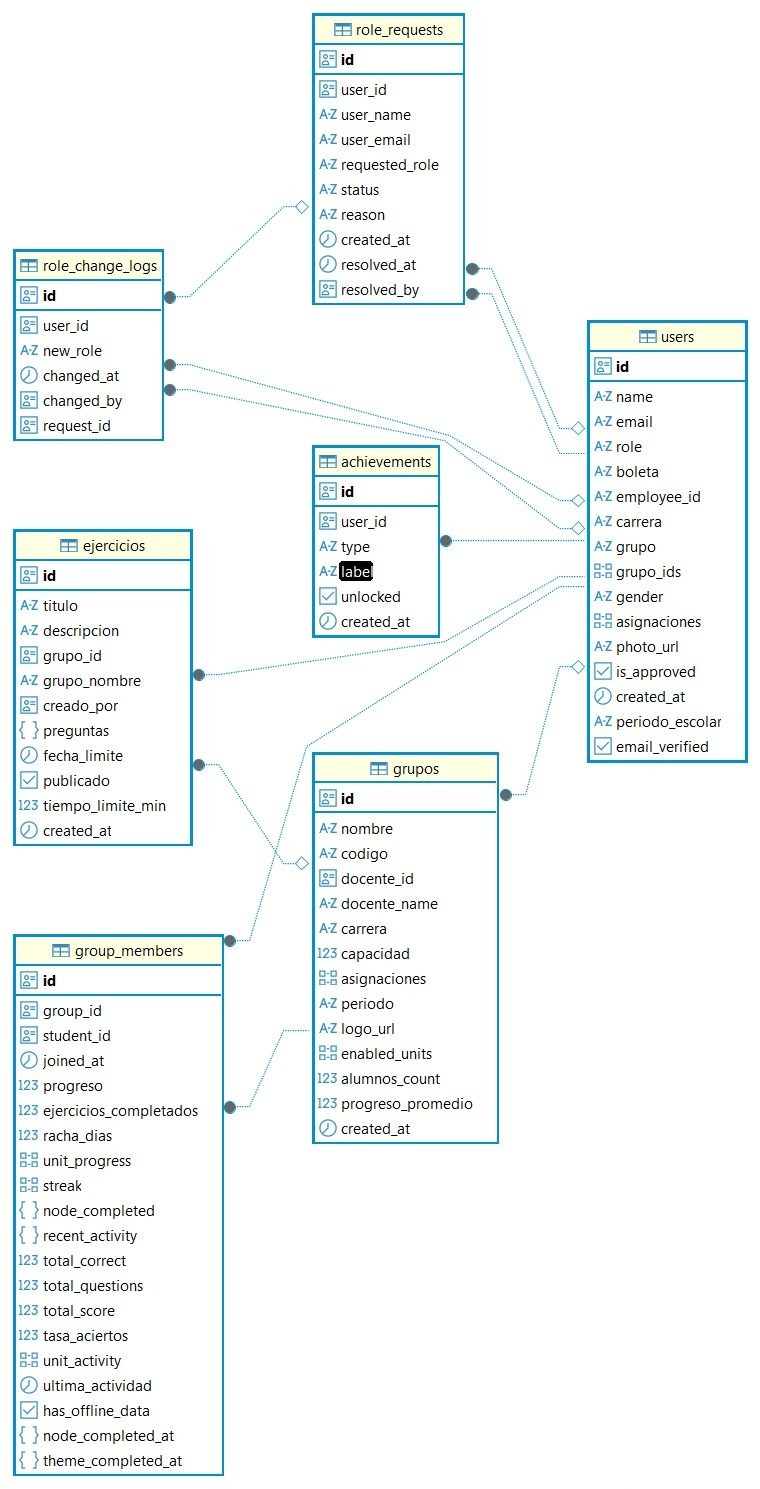
\includegraphics[width=0.70\textwidth]{imagenes/DiagramaER.jpg} % <--- Asegúrate de que tu imagen esté en esta ruta y formato
    \caption{Diagrama Entidad-Relación del esquema físico PostgreSQL de AUTECH, mostrando las entidades \texttt{users}, \texttt{grupos}, \texttt{group\_members}, \texttt{ejercicios}, \texttt{role\_requests} y \texttt{achievements} con sus relaciones y atributos principales.}
    \label{fig:diagrama_er}
\end{figure}

\subsection{Modelado Detallado por Módulos (UML)}
\label{subsec:modelado_modular_uml}

A continuación, se presenta el desglose analítico e interactivo del sistema AUTECH organizado por cada uno de sus módulos arquitectónicos. Para cada bloque, se detalla el alcance mediante diagramas de casos de uso y se justifica la transferencia temporal de mensajes mediante diagramas de secuencia específicos, alineados de forma estricta con la secuencia numérica consolidada.

\subsubsection{Módulo I: Autenticación, Seguridad y Accesos (Transversal)}

Este módulo norma el ingreso seguro y la persistencia de la sesión mediante los servicios distribuidos de Supabase Auth. El alcance de sus interacciones (desde el registro del Alumno hasta las solicitudes de aprovisionamiento de los Docentes) se ilustra en la Figura~\ref{fig:dcu_modulo_1}.

\begin{figure}[htbp]
    \centering
    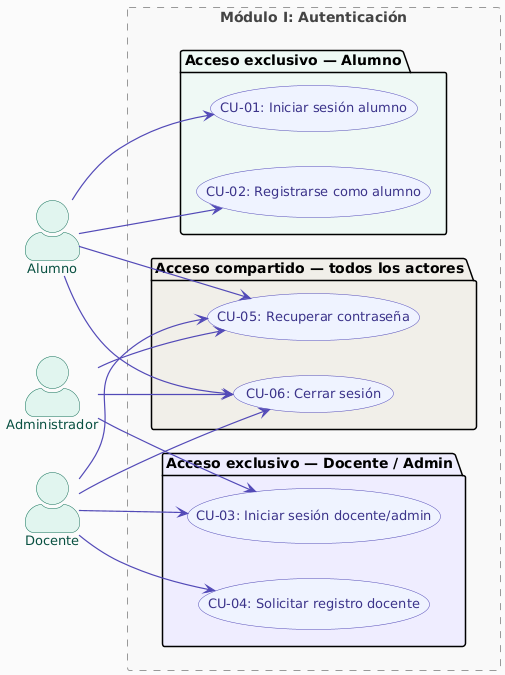
\includegraphics[width=0.85\textwidth]{imagenes/dcu_m1_auth.png}
    \caption{Diagrama de Casos de Uso del Módulo de Autenticación, Seguridad y Accesos.}
    \label{fig:dcu_modulo_1}
\end{figure}

Para validar el flujo síncrono de verificación y el intercambio de \textit{JSON Web Tokens} (JWT) entre el cliente multiplataforma y la infraestructura en la nube, se desarrolló el diagrama de secuencia expuesto en la Figura~\ref{fig:seq_m1_login}.

\begin{figure}[htbp]
    \centering
    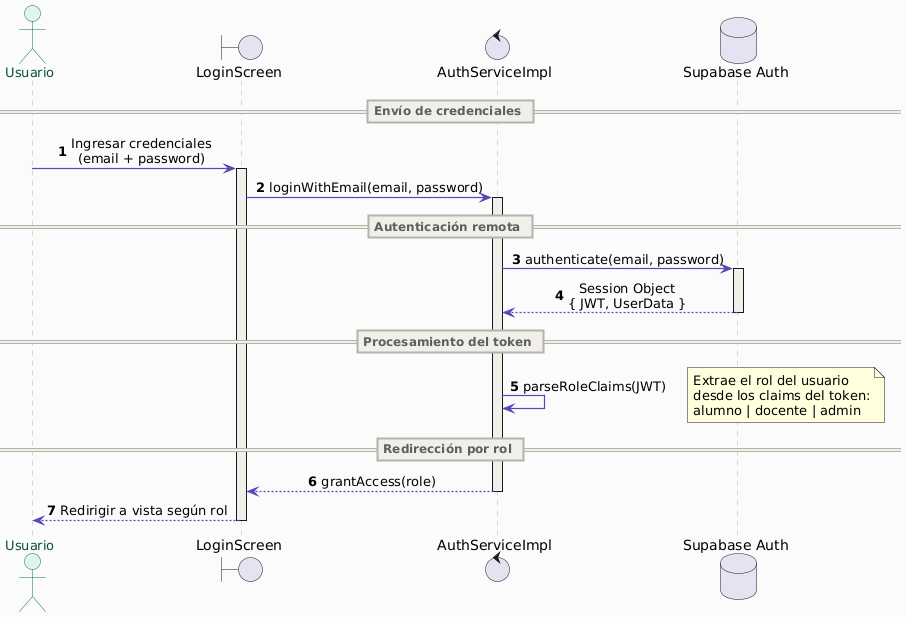
\includegraphics[width=0.95\textwidth]{imagenes/seq_m1_login.png}
    \caption{Diagrama de Secuencia para el inicio de sesión unificado y validación de roles.}
    \label{fig:seq_m1_login}
\end{figure}

\paragraph{Análisis del Comportamiento Dinámico (CU-01 / CU-03):}~\\
El flujo de interacción inicia cuando el usuario introduce sus credenciales en la interfaz \texttt{LoginScreen}. La vista delega el control a la capa de negocio invocando el método asíncrono \texttt{loginWithEmail()} de la implementación \texttt{AuthServiceImpl}. Esta clase actúa como pasarela enviando una petición cifrada vía HTTPS a la API remota de \texttt{Supabase Auth}. 

Tras validar las credenciales en la base de datos central, el servidor retorna un objeto de sesión atómico que encapsula un token de acceso firmado (JWT) y los metadatos de identidad. Finalmente, la lógica del servicio desencadena un mapeo interno para decodificar los \textit{role claims} del token, persistir de forma segura la sesión localmente y enrutar reactivamente al usuario hacia la interfaz correspondiente a su rol, garantizando el aislamiento de privilegios.

\subsubsection{Módulo II: Núcleo de Simulación, Algoritmos y Aprendizaje (Alumno)}

Representa el motor computacional de AUTECH en el cliente móvil. Este módulo administra la lógica matemática abstracta de la jerarquía de lenguajes formales. En la Figura~\ref{fig:dcu_modulo_2} se delimita el alcance de las herramientas interactivas del lienzo táctil, conversiones y resolución de retos didácticos.

\begin{figure}[htbp]
    \centering
    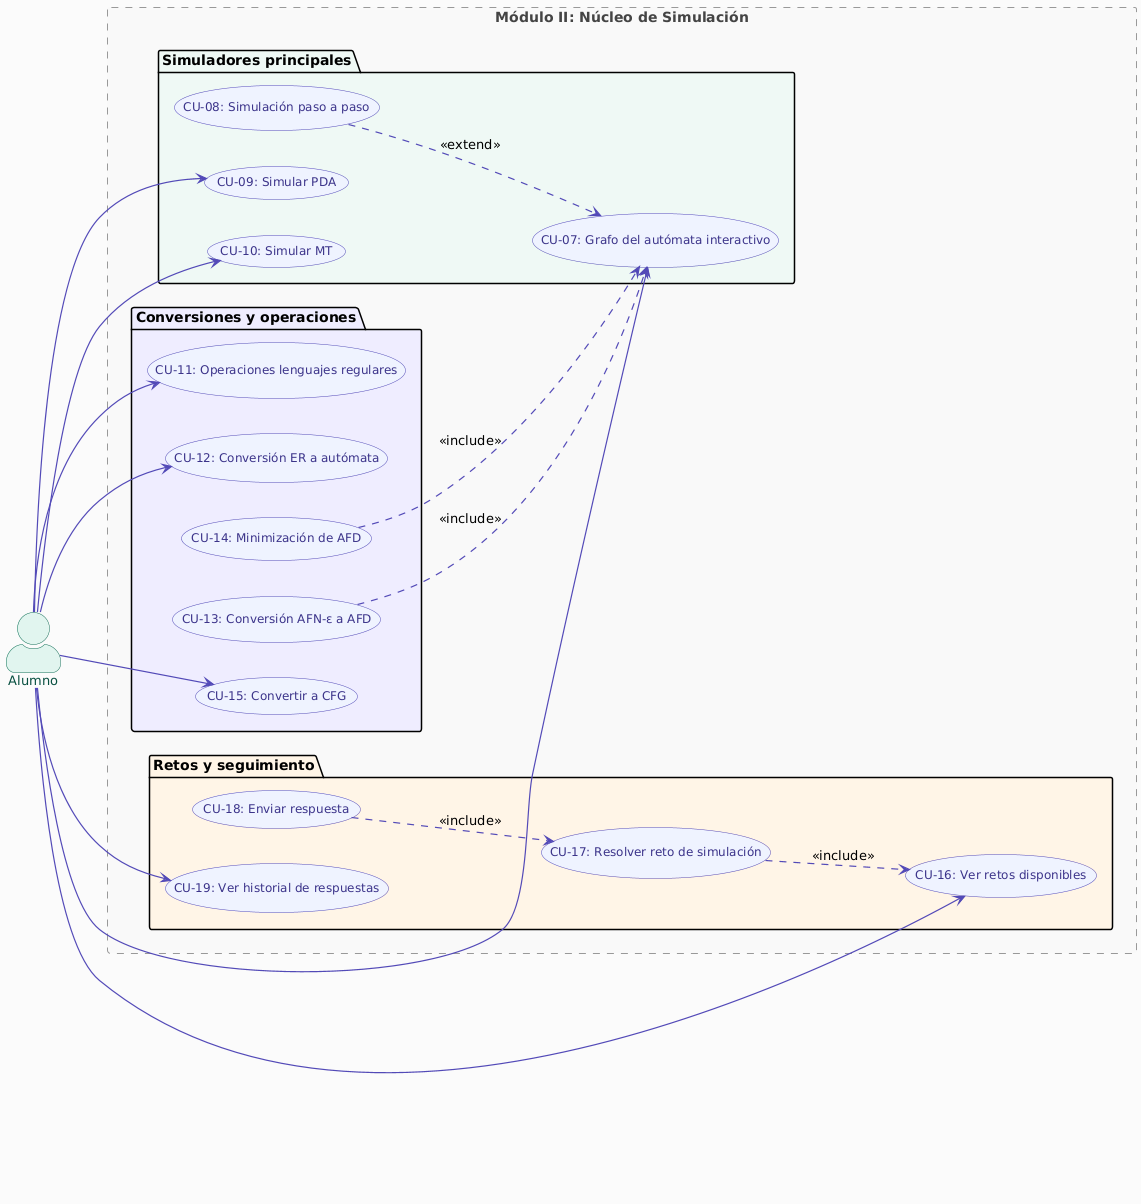
\includegraphics[width=0.90\textwidth]{imagenes/dcu_m2_simulacion.png}
    \caption{Diagrama de Casos de Uso del Núcleo de Simulación, Algoritmos y Aprendizaje.}
    \label{fig:dcu_modulo_2}
\end{figure}

Debido a su alta complejidad algorítmica, se modelaron dos interacciones críticas de procesamiento en memoria volátil:

\begin{figure}[htbp]
    \centering
    \includegraphics[width=0.95\textwidth]{imagenes/seq_m2_conversion.png}
    \caption{Diagrama de Secuencia del Motor Algorítmico para la transformación formal de autómatas.}
    \label{fig:seq_m2_conversion}
\end{figure}

\paragraph{Análisis del Comportamiento Dinámico - Conversión (CU-13):}~\\
Como se aprecia en la Figura~\ref{fig:seq_m2_conversion}, el proceso arranca cuando el Alumno solicita la transformación estructural en el lienzo interactivo. La clase de la vista invoca la rutina de conversión \texttt{ejecutarConversion()} expuesta por el componente especializado \texttt{ChomskyConverterImpl}. Para eliminar el no-determinismo provocado por transiciones vacías, el convertidor interactúa cíclicamente con el componente de bajo nivel \texttt{AutomataEngineImpl} mediante la llamada \texttt{calcularLambdaClausura()}. 

El motor matemático evalúa el grafo y retorna el subconjunto de clausuras elementales. Con esta información, el convertidor ejecuta el Algoritmo de Construcción de Subconjuntos en memoria volátil para derivar una tabla de transiciones unívoca. Una vez consolidada la nueva estructura matemática del AFD resultante, se invoca al componente \texttt{AutomataRepository} para almacenar permanentemente la topología en el almacenamiento local y notificar reactivamente al canvas gráfico para refrescar el renderizado visual de los nodos y aristas a 60 FPS.

\begin{figure}[htbp]
    \centering
    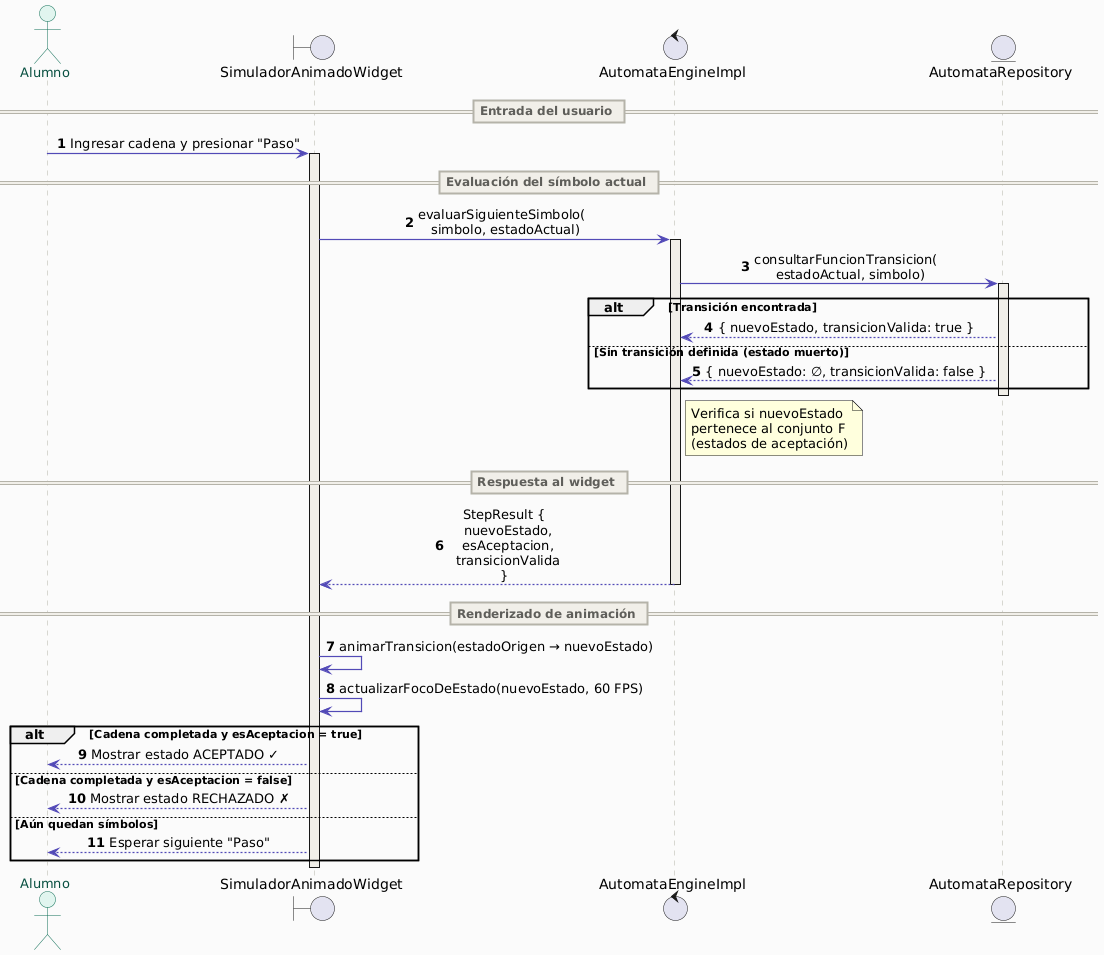
\includegraphics[width=0.95\textwidth]{imagenes/seq_m2_paso.png}
    \caption{Diagrama de Secuencia para la ejecución paso a paso de cadenas en el lienzo interactivo.}
    \label{fig:seq_m2_paso}
\end{figure}

\paragraph{Análisis del Comportamiento Dinámico - Simulación Paso a Paso (CU-08):}~\\
El ciclo dinámico detallado en la Figura~\ref{fig:seq_m2_paso} describe la traza de evaluación de cadenas de entrada. Al activar la ejecución paso a paso, el widget \texttt{SimuladorAnimadoWidget} extrae secuencialmente los símbolos del alfabeto de entrada y los transmite al motor algorítmico a través de la instrucción \texttt{evaluarSiguienteSimbolo()}. El motor consulta asíncronamente con el repositorio de datos (\texttt{AutomataRepository}) el mapeo de la función de transición $\delta(q, \sigma)$. 

Si la combinación de estado actual y símbolo de entrada es válida, el repositorio devuelve la configuración de destino. El motor procesa el cambio de estado latente y responde a la interfaz con la metadata de la transición autorizada. Finalmente, el widget intercepta el mensaje y ejecuta de forma reactiva las animaciones sobre el lienzo matemático, resaltando el nodo activo y la arista recorrida para facilitar al alumno el rastreo lógico de la simulación.

\subsubsection{Módulo III: Sincronización y Persistencia (Arquitectura Offline)}

Este módulo funge como un \textit{middleware} reactivo que garantiza la tolerancia a fallas de red en la aplicación móvil. Sus interacciones, orientadas a conmutar de forma transparente entre la base de datos local Hive y Supabase, se modelan en la Figura~\ref{fig:dcu_modulo_3}.

\begin{figure}[htbp]
    \centering
    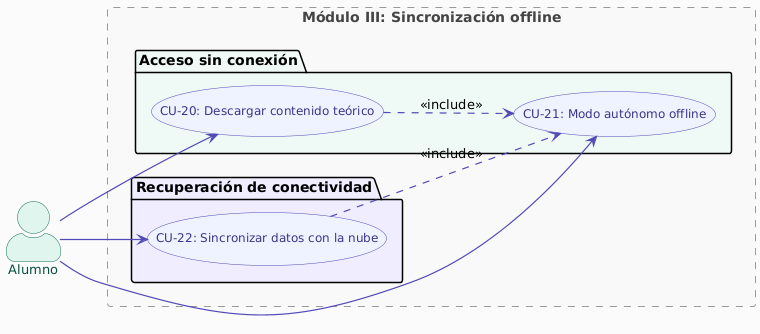
\includegraphics[width=0.85\textwidth]{imagenes/dcu_m3_offline.png}
    \caption{Diagrama de Casos de Uso del Módulo de Sincronización y Persistencia Offline.}
    \label{fig:dcu_modulo_3}
\end{figure}

El proceso temporal de encolamiento asíncrono e interceptación de conectividad para el volcado atómico de datos (\textit{Bulk Write}) al recuperar enlace con la nube (CU-22) se detalla rigurosamente en la Figura~\ref{fig:seq_m3_sync}.

\begin{figure}[htbp]
    \centering
    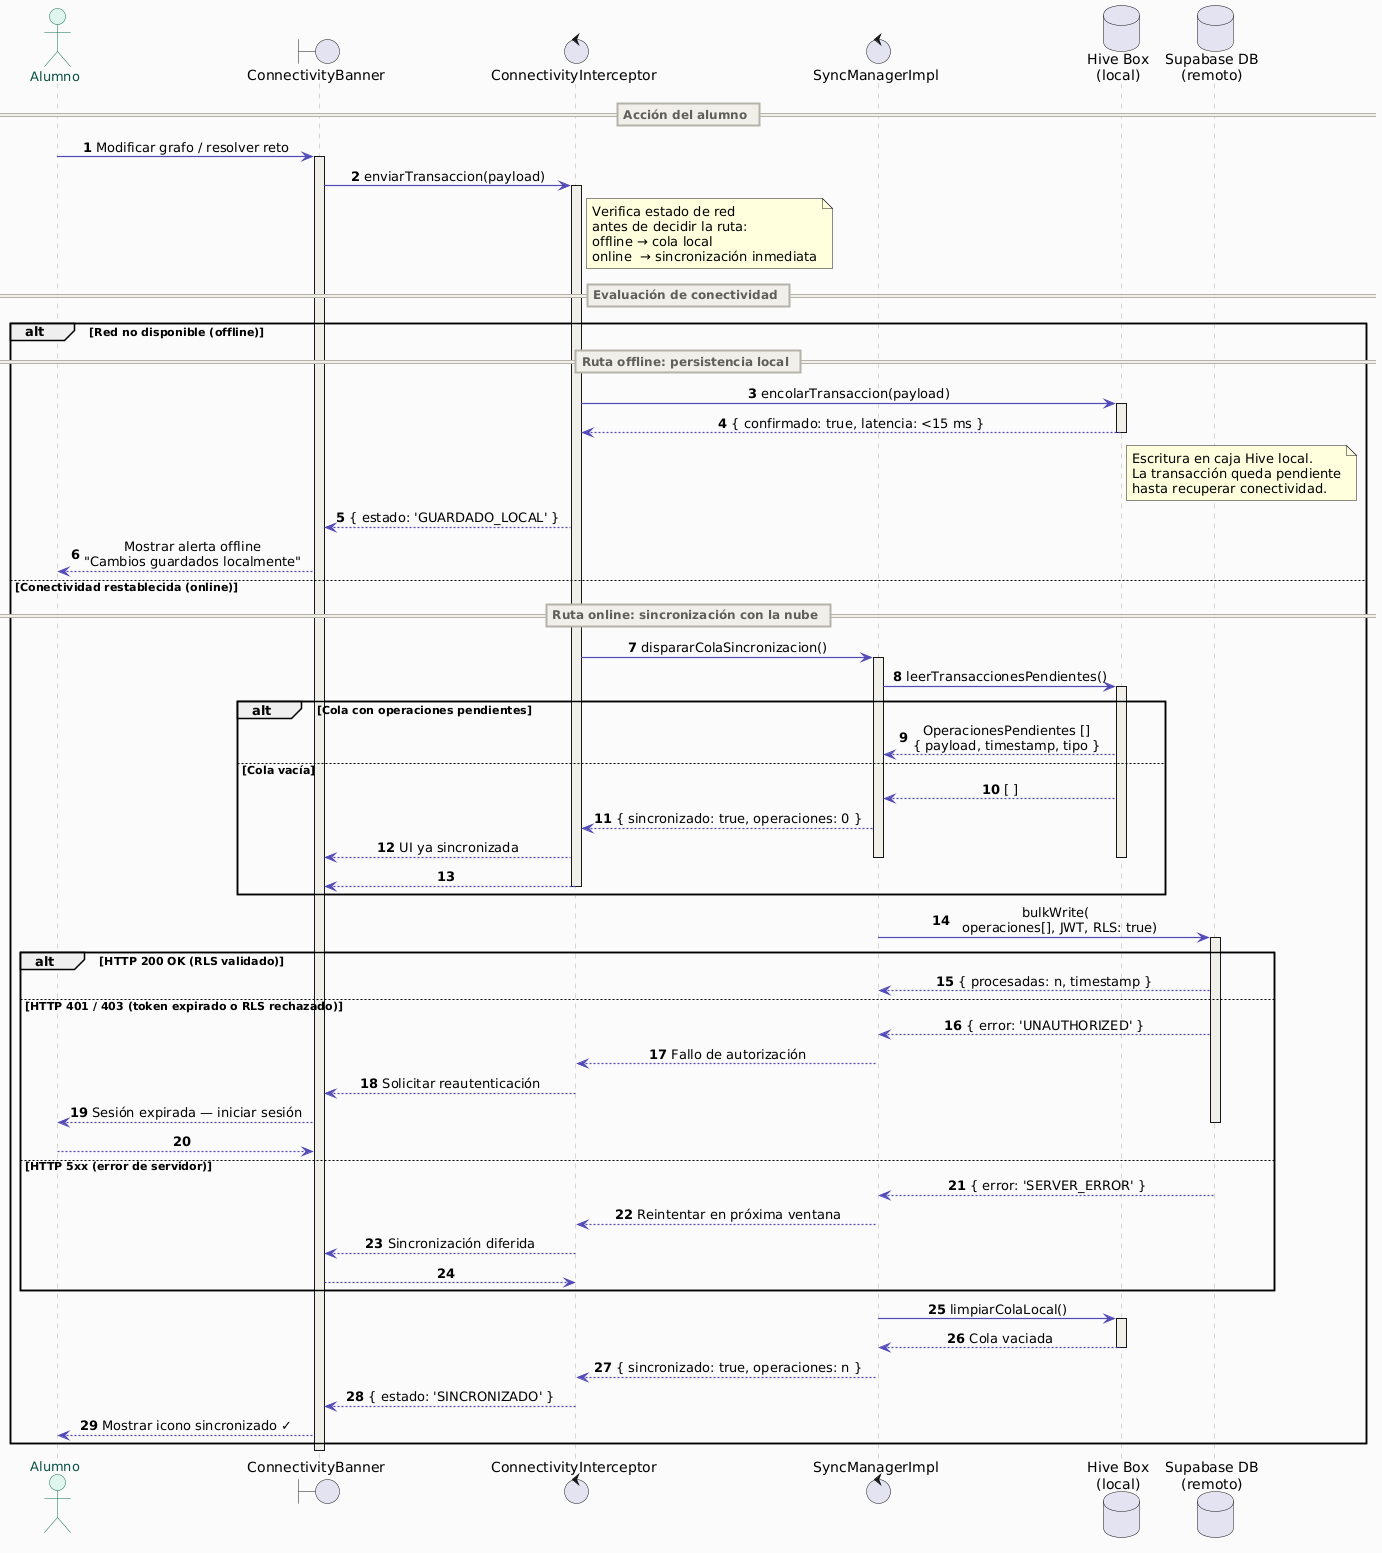
\includegraphics[width=0.95\textwidth]{imagenes/seq_m3_sincronizacion.png}
    \caption{Diagrama de Secuencia del flujo de Sincronización Asíncrona con la capa remota.}
    \label{fig:seq_m3_sync}
\end{figure}

\paragraph{Análisis del Comportamiento Dinámico (CU-22):}~\\
La dinámica transaccional expuesta en la Figura~\ref{fig:seq_m3_sync} sustenta la resiliencia offline de la aplicación móvil. Al registrarse interacciones didácticas, el componente reactivo \texttt{ConnectivityInterceptor} monitoriza el estado físico de los adaptadores de red del dispositivo. Si el interceptor detecta la ausencia de conectividad, desvía inmediatamente el flujo de datos fuera del flujo remoto de internet e invoca un guardado local imperativo en las cajas estructuradas de \texttt{Hive Box}. Hive procesa la serialización en formato binario garantizando latencias de escritura de bajísimo impacto ($< 15$ ms) y devuelve un estado de confirmación para alertar sutilmente al usuario en la UI.

En el instante en que el interceptor registra la reconexión exitosa a internet, dispara de manera automatizada el proceso de vaciado invocando al componente central \texttt{SyncManagerImpl}. Este gestor extrae en ráfaga las operaciones encoladas en Hive en formato JSON y orquesta una petición unificada hacia la base de datos PostgreSQL en la nube de \texttt{Supabase}. Tras verificarse de forma exitosa las políticas de seguridad a nivel de fila (RLS), el backend remoto consolida los registros de progreso devolviendo un código HTTP 200 OK. Finalmente, el gestor purga la memoria local de Hive y actualiza el estado visual a ``Sincronizado''.

\subsubsection{Módulo IV: Experiencia de Usuario y Ludificación (Alumno)}

Encargado de los incentivos visuales y mecánicas formativas que impulsan la retención del estudiante. Su alcance operativo e interacciones con el catálogo de logros se presentan en la Figura~\ref{fig:dcu_modulo_4}.

\begin{figure}[htbp]
    \centering
    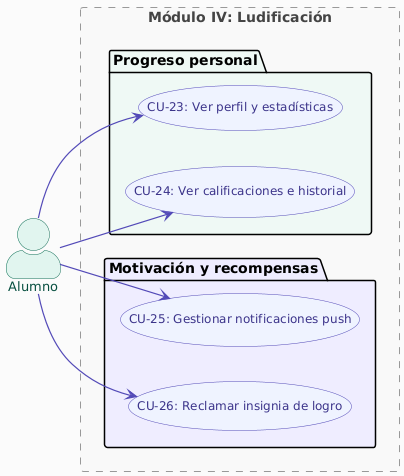
\includegraphics[width=0.85\textwidth]{imagenes/dcu_m4_ludificacion.png}
    \caption{Diagrama de Casos de Uso del Módulo de Experiencia de Usuario y Ludificación.}
    \label{fig:dcu_modulo_4}
\end{figure}

En la Figura~\ref{fig:seq_m4_logro} se describe el flujo de eventos desencadenado tras resolver un ejercicio exitosamente, justificando el procesamiento local de rachas y la posterior persistencia síncrona de insignias desbloqueadas (CU-26).

\begin{figure}[htbp]
    \centering
    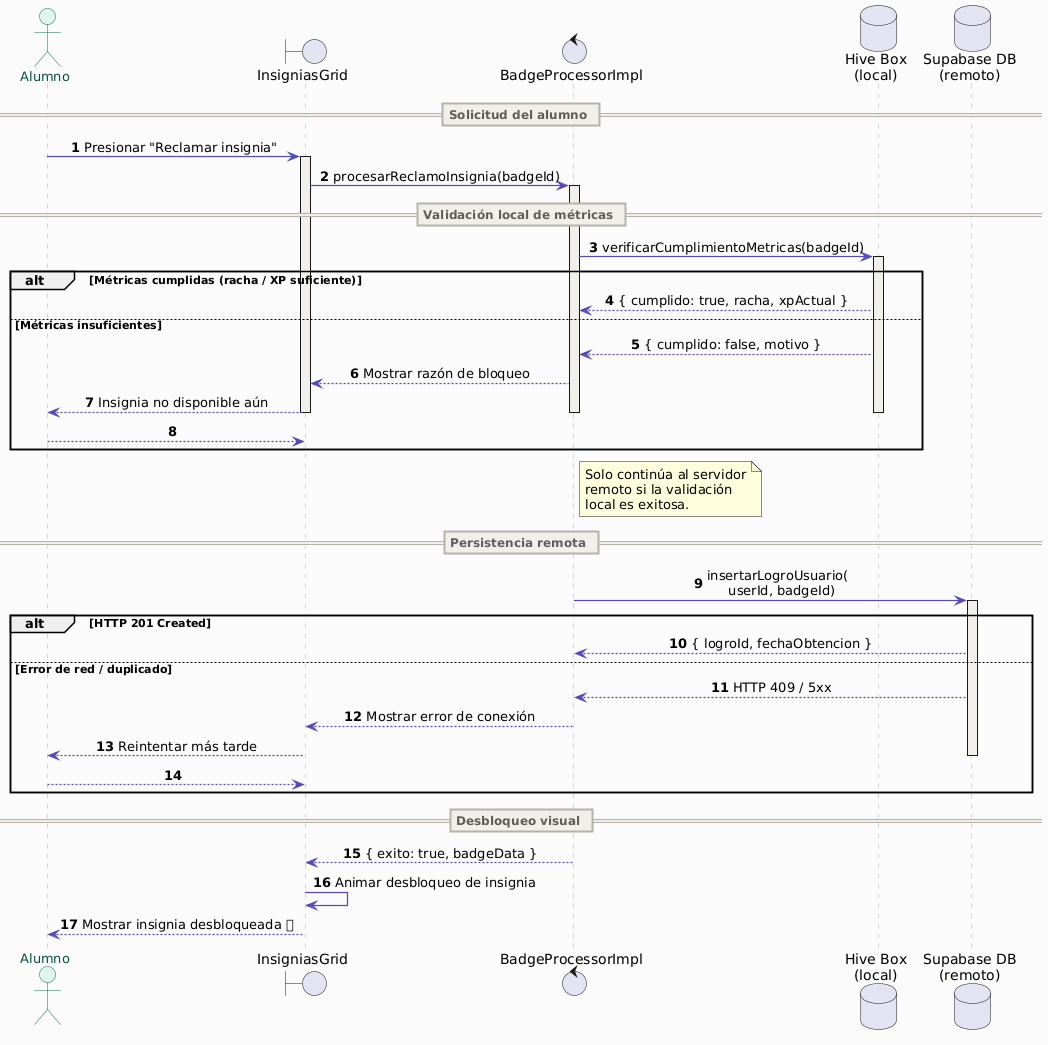
\includegraphics[width=0.95\textwidth]{imagenes/seq_m4_logro.png}
    \caption{Diagrama de Secuencia del Motor de Ludificación para la asignación y reclamo de insignias.}
    \label{fig:seq_m4_logro}
\end{figure}

\paragraph{Análisis del Comportamiento Dinámico (CU-26):}~\\
Como se ilustra en la Figura~\ref{fig:seq_m4_logro}, el ciclo de gamificación se activa de manera síncrona cuando el Alumno presiona el botón de reclamo en la vista \texttt{InsigniasGrid}. El widget delega el procesamiento lúdico al componente de negocio \texttt{BadgeProcessorImpl} invocando el método \texttt{procesarReclamoInsignia()}. El procesador realiza una validación cruzada consultando las métricas históricas de rendimiento persistidas localmente en \texttt{Hive Storage}. 

Si las cajas locales certifican que el usuario cumple con los umbrales específicos del logro (como el contador de racha de estudio o puntos de experiencia XP acumulados), el procesador autoriza la transacción y emite un comando de inserción hacia la tabla de perfiles de \texttt{Supabase DB}. Al retornar el código HTTP 201 de persistencia exitosa desde la nube, el componente del servicio libera el candado visual de la insignia y refresca la UI, otorgándole al estudiante retroalimentación inmediata sobre su progreso didáctico.

\subsubsection{Módulo V: Dashboard de Gestión Docente (Plataforma Desktop)}

Herramienta analítica y de control didáctico exclusiva del profesor. La definición de sus funciones para la edición de reactivos y el consumo de reportes e indicadores grupales se detalla en la Figura~\ref{fig:dcu_modulo_5}.

\begin{figure}[htbp]
    \centering
    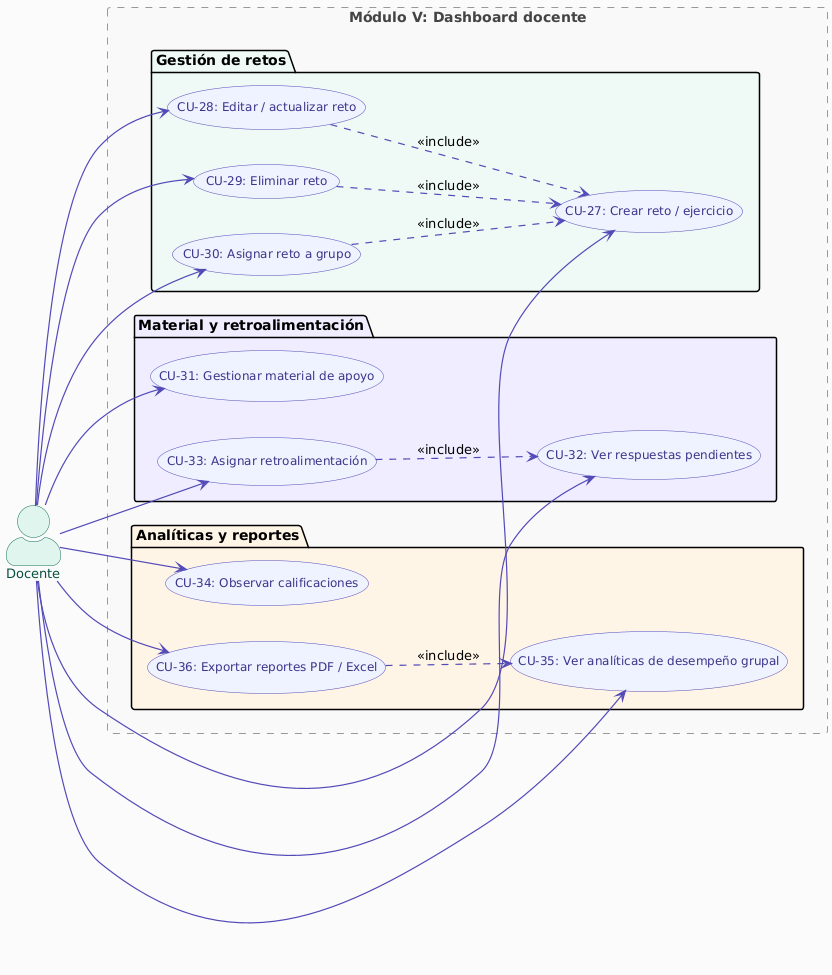
\includegraphics[width=0.90\textwidth]{imagenes/dcu_m5_docente.png}
    \caption{Diagrama de Casos de Uso del Dashboard de Gestión Docente.}
    \label{fig:dcu_modulo_5}
\end{figure}

La Figura~\ref{fig:seq_m5_analiticas} expone de forma secuencial cómo el Dashboard Desktop consume las funciones remotas (RPC) y vistas optimizadas de Supabase para generar semáforos de desempeño grupal en tiempo real de manera asíncrona (CU-35).

\begin{figure}[htbp]
    \centering
    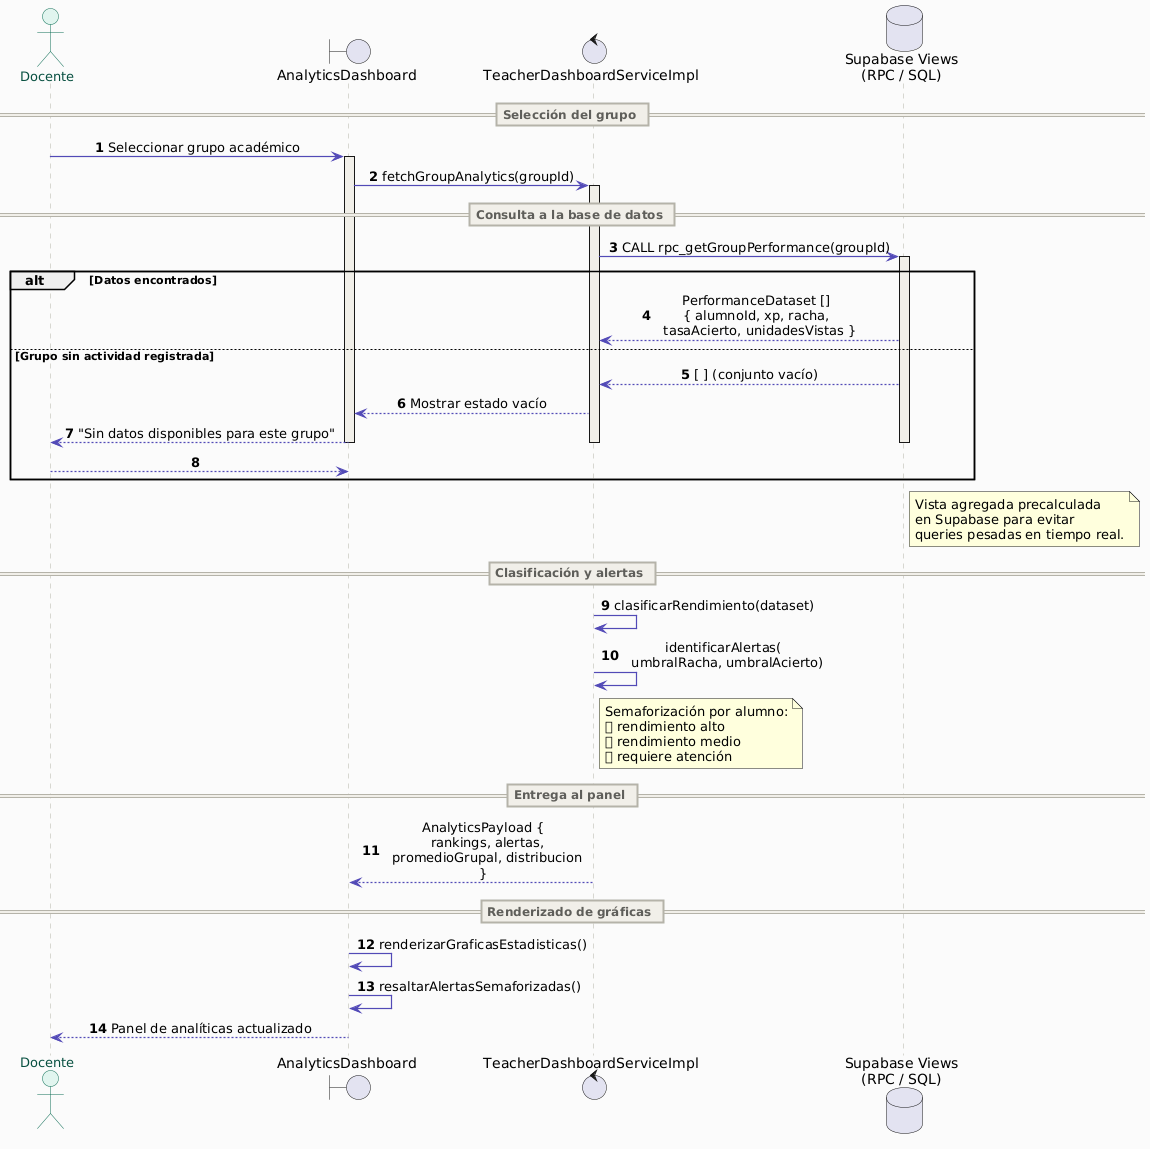
\includegraphics[width=0.95\textwidth]{imagenes/seq_m5_analiticas.png}
    \caption{Diagrama de Secuencia para la consulta reactiva y renderizado de métricas analíticas.}
    \label{fig:seq_m5_analiticas}
\end{figure}

\paragraph{Análisis del Comportamiento Dinámico (CU-35):}~\\
El flujo analítico modelado en la Figura~\ref{fig:seq_m5_analiticas} detalla el procesamiento de métricas de evaluación formativa. Cuando el profesor selecciona un grupo escolar en el panel administrativo \texttt{AnalyticsDashboard}, el entorno web/desktop gatilla una llamada asíncrona hacia el controlador \texttt{TeacherDashboardServiceImpl} por medio de la rutina \texttt{fetchGroupAnalytics()}. El servicio canaliza la consulta de manera directa hacia la capa de datos de Supabase, invocando un procedimiento almacenado (\textit{Remote Procedure Call} - RPC) configurado sobre la base de datos PostgreSQL.

La base de datos ejecuta de forma interna las agregaciones matemáticas sobre los históricos de respuestas y retorna un objeto estructurado JSON que contiene las métricas procesadas. El servicio de la plataforma docente captura la respuesta, mapea las variables de rendimiento y evalúa los umbrales estipulados para semaforizar los indicadores (alertas en rojo, amarillo o verde). Finalmente, el dataset formateado se transmite de vuelta a la UI, pintando gráficos estadísticos que facilitan la toma de decisiones pedagógicas al docente.

\subsubsection{Módulo I\MakeUppercase{V}: Gestión Administrativa Global (Consola Admin)}

Módulo operativo de máximo nivel jerárquico. Administra catálogos maestros, auditoría de logs y aprovisionamiento institucional. Su alcance se modela en la Figura~\ref{fig:dcu_modulo_6}.

\begin{figure}[htbp]
    \centering
    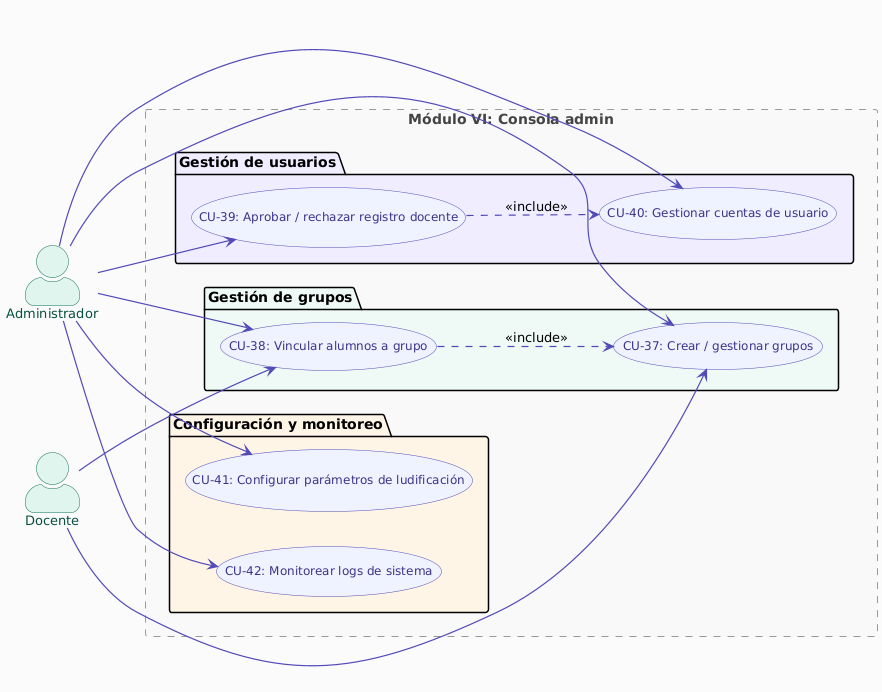
\includegraphics[width=0.85\textwidth]{imagenes/dcu_m6_admin.png}
    \caption{Diagrama de Casos de Uso del Módulo de Gestión Administrativa Global.}
    \label{fig:dcu_modulo_6}
\end{figure}

Finalmente, la Figura~\ref{fig:seq_m6_aprobacion} detalla el flujo crítico de seguridad para la validación y autorización del registro de un nuevo docente (CU-39), manipulando los estados de las tablas maestras bajo aislamiento transaccional.

\begin{figure}[htbp]
    \centering
    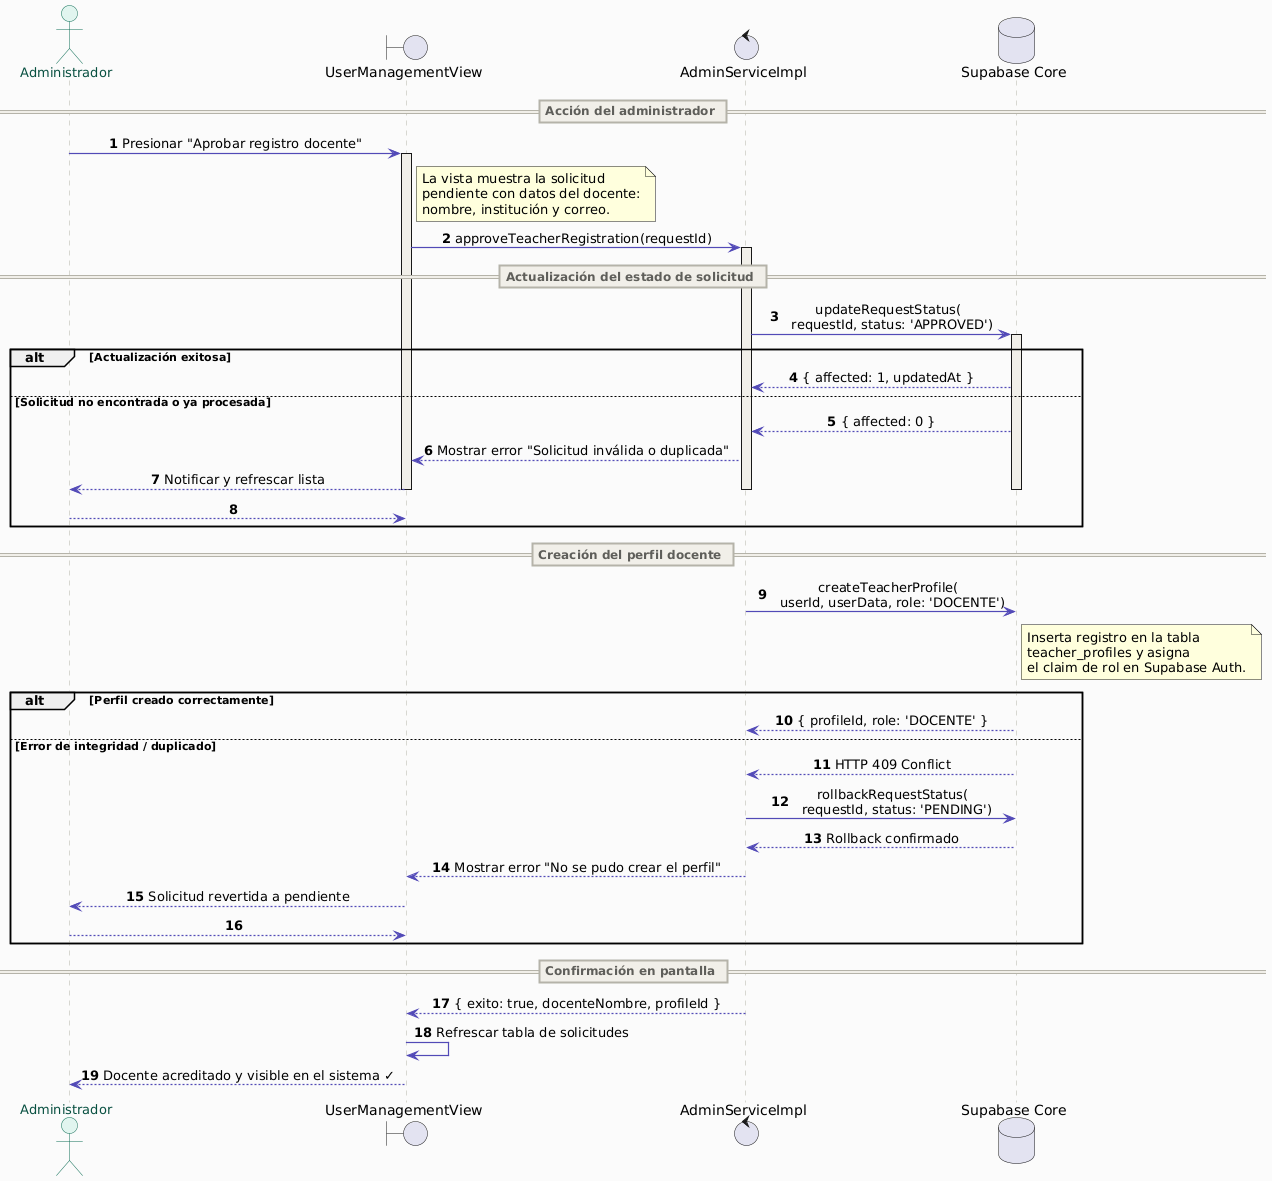
\includegraphics[width=0.95\textwidth]{imagenes/seq_m6_aprobacion.png}
    \caption{Diagrama de Secuencia para el flujo de Aprobación/Rechazo de credenciales docentes.}
    \label{fig:seq_m6_aprobacion}
\end{figure}

\paragraph{Análisis del Comportamiento Dinámico (CU-39):}~\\
La traza temporal descrita en la Figura~\ref{fig:seq_m6_aprobacion} gobierna el aprovisionamiento de identidades institucionales de alto nivel. Al activarse la opción de autorización en la consola maestra (\texttt{UserManagementView}), el Administrador delega la lógica crítica de seguridad al componente de control \texttt{AdminServiceImpl} invocando la función \texttt{approveTeacherRegistration()}. El servicio abre inmediatamente un bloque transaccional seguro y altera el registro correspondiente en la tabla de solicitudes de Supabase, conmutando su estado a ``APPROVED''.

Una vez validada esta mutación de datos por el motor de PostgreSQL, el servicio lanza de forma secuencial una segunda instrucción dirigida al esquema central de autenticación para dar de alta el perfil docente definitivo e inyectar de manera segura el rol RBAC verificado. Al completarse con éxito ambas operaciones, la base de datos consolida el cambio transaccional de forma permanente y responde al servicio. Finalmente, el componente administrativo refresca de forma síncrona la vista de control reflejando el nuevo estatus del usuario en los paneles del sistema.